\documentclass[12pt]{ximera}
\title{Exam 3 (2020)}
\begin{document}
\begin{abstract}
An archived exam on Chapter 3, with its take-home part: lone-divider bids, a three-flavor sub, divider-chooser on a pizza, sealed bids in a divorce, and resolving a standoff.
\end{abstract}
\maketitle

\section*{Exam 3 (2020)}

\begin{problem}
Alice, the Cheshire Cat, the White Rabbit, and the Mad Hatter are dividing the leftovers
from tea time, which they own equally. One of them has divided the assets into four shares.
The table shows each player's value for each share, as a percent of the total.
\begin{center}
\begin{tabular}{|c|c|c|c|c|}\hline
 & $s_1$ & $s_2$ & $s_3$ & $s_4$\\\hline
Alice & 20\% & 32\% & 28\% & 20\%\\\hline
Cheshire Cat & 25\% & 25\% & 25\% & 25\%\\\hline
White Rabbit & 15\% & 15\% & 30\% & 40\%\\\hline
Mad Hatter & 24\% & 26\% & 24\% & 26\%\\\hline
\end{tabular}
\end{center}

\begin{prompt}
\textbf{(a)} Who was the divider?
\begin{multipleChoice}
\choice{Alice}
\choice[correct]{The Cheshire Cat}
\choice{The White Rabbit}
\choice{The Mad Hatter}
\end{multipleChoice}
\begin{feedback}
Only the Cheshire Cat values all four shares equally, at exactly $25\%$.
\end{feedback}
\end{prompt}

\begin{prompt}
\textbf{(b)} In every fair division, which share does the Cheshire Cat receive?
share number $\answer{1}$

\smallskip
How many fair divisions are there in total? $\answer{2}$
\begin{feedback}
Fair shares (at least $25\%$): Alice $\set{s_2,s_3}$, White Rabbit $\set{s_3,s_4}$,
Mad Hatter $\set{s_2,s_4}$, Cheshire Cat any. Nobody but the Cheshire Cat wants $s_1$.
The other three form a cycle, which can be resolved in two ways:
\begin{itemize}
\item Alice $s_2$, White Rabbit $s_3$, Mad Hatter $s_4$, Cheshire Cat $s_1$;
\item Alice $s_3$, White Rabbit $s_4$, Mad Hatter $s_2$, Cheshire Cat $s_1$.
\end{itemize}
\end{feedback}
\end{prompt}
\end{problem}

\begin{problem}
Lisa, Bart, and Homer jointly bought a giant $21$-inch sub for \$12. From left to right,
the sandwich is $7$ inches of chicken, $7$ inches of tuna, and $7$ inches of vegetarian.
Lisa likes all three flavors equally well. Bart likes chicken three times as much as
vegetarian and tuna twice as much as vegetarian. Homer likes tuna twice as much as
chicken and hates vegetarian.

\begin{prompt}
\textbf{(a)} Give each player's value system, as fractions of the whole sub.

Bart --- chicken $\answer{1/2}$, tuna $\answer{1/3}$, veggie $\answer{1/6}$

\smallskip
Homer --- chicken $\answer{1/3}$, tuna $\answer{2/3}$, veggie $\answer{0}$
\begin{feedback}
Bart's ratio $3:2:1$ gives $\frac36,\frac26,\frac16$; Homer's $1:2:0$ gives
$\frac13,\frac23,0$. Lisa values each flavor at $\frac13$.
\end{feedback}
\end{prompt}

\begin{prompt}
\textbf{(b)} If Homer is the lone divider, where does he make his two cuts, in inches
from the left?

First cut: $\answer{7}$ \quad Second cut: $\answer{10.5}$
\begin{feedback}
Each share must be worth $\frac13$ to Homer. The chicken alone is worth $\frac13$, so
$s_1=[0,7]$. The tuna is worth $\frac23$, so it is cut in half: $s_2=[7,10.5]$, and
$s_3=[10.5,21]$ is the other half of the tuna plus the veggie, which Homer thinks is
worthless.
\end{feedback}
\end{prompt}

\begin{prompt}
\textbf{(c)} Suppose instead that Bart is the divider, with shares
$s_1=[0,\tfrac{14}3]$, $s_2=[\tfrac{14}3,10.5]$, and $s_3=[10.5,21]$. What is each share
worth to Lisa?

$s_1$: $\answer{2/9}$ \quad $s_2$: $\answer{5/18}$ \quad $s_3$: $\answer{1/2}$

\smallskip
So Lisa bids only for share number $\answer{3}$.
\begin{feedback}
Lisa values the sub by length: $\frac{14/3}{21}=\frac29$,
$\frac{10.5-14/3}{21}=\frac{35/6}{21}=\frac5{18}$, and $\frac{10.5}{21}=\frac12$. Only
$s_3$ is at least $\frac13$.
\end{feedback}
\end{prompt}

\begin{prompt}
\textbf{(d)} Homer bids $\set{s_2,s_3}$. Describe the fair division and its dollar values.

Bart gets share number $\answer{1}$, worth \$$\answer{4}$ to him.

\smallskip
Lisa gets share number $\answer{3}$, worth \$$\answer{6}$ to her.

\smallskip
Homer gets share number $\answer{2}$, worth \$$\answer[tolerance=0.005]{5.33}$ to him.
\begin{feedback}
Lisa must have $s_3$, so Homer takes $s_2$ and Bart, the divider, takes $s_1$, worth
$\frac13\cdot\$12=\$4$ to him. Lisa's $s_3$ is worth $\frac12\cdot\$12=\$6$.

Homer's $s_2$ holds $7-\frac{14}3=\frac73$ inches of chicken, worth
$\frac{7/3}{7}\cdot\frac13=\frac19$, and $3.5$ inches of tuna, worth
$\frac12\cdot\frac23=\frac13$. That is $\frac49$ of the sub, or
$\frac49\cdot\$12\approx\$5.33$.
\end{feedback}
\end{prompt}
\end{problem}

\begin{problem}
Sheldon and Penny split the pizza they bought for lunch using the divider-chooser method.
The pizza is $\frac13$ sausage, $\frac13$ mushroom, and $\frac13$ olive:
\begin{center}
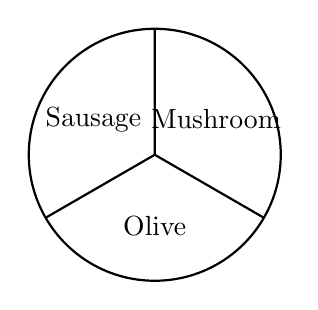
\begin{tikzpicture}
\draw[thick] (0,0) circle (1.6);
\draw[thick] (0,0) -- (90:1.6) (0,0) -- (210:1.6) (0,0) -- (330:1.6);
\node at (150:0.9) {Sausage};
\node at (30:0.9) {Mushroom};
\node at (270:0.9) {Olive};
\end{tikzpicture}
\end{center}
Sheldon likes sausage and mushroom equally but hates olives. Penny likes mushroom and
olive equally but doesn't eat sausage. Penny lost a game of rock-paper-scissors and is
the divider.

\begin{prompt}
\textbf{(a)} What is each topping worth to Penny?

Sausage $\answer{0}$ \quad Mushroom $\answer{1/2}$ \quad Olive $\answer{1/2}$
\begin{feedback}
She values mushroom and olive equally and sausage not at all.
\end{feedback}
\end{prompt}

\begin{prompt}
\textbf{(b)} Which of these cuts are acceptable for Penny, the divider?
\begin{selectAll}
\choice[correct]{$s_1=$ sausage $+$ mushroom, $s_2=$ olive}
\choice{$s_1=$ sausage, $s_2=$ mushroom $+$ olive}
\choice[correct]{$s_1=$ mushroom $+$ half the sausage, $s_2=$ olive $+$ half the sausage}
\choice{$s_1=$ mushroom $+$ olive, $s_2=$ sausage}
\end{selectAll}
\begin{feedback}
Penny must cut two shares worth $\frac12$ each to her, which means the mushroom and the
olive go to different shares. The sausage is worth nothing to her, so it can go
anywhere.
\end{feedback}
\end{prompt}

\begin{prompt}
\textbf{(c)} Penny cuts along the slice lines: $s_1=$ sausage $+$ mushroom and $s_2=$
olive. Which share does Sheldon pick, and what is it worth to him?

Sheldon picks share number $\answer{1}$, worth $\answer{1}$ (as a fraction of the pizza's value to him)
\begin{feedback}
Sheldon values sausage and mushroom at $\frac12$ each and olive at $0$, so $s_1$ is
worth $100\%$ to him and $s_2$ nothing. Both players come out well: Sheldon gets
everything he values, and Penny gets exactly half of what she values.
\end{feedback}
\end{prompt}
\end{problem}

\begin{problem}
A divorcing couple, Ana and Ben, share some items with sentimental value. Instead of
selling them, they use the method of sealed bids.
\begin{center}
\begin{tabular}{|l|r|r|}\hline
 & \textbf{Ana} & \textbf{Ben}\\\hline
House & \$2,100,000 & \$2,198,000\\
Armored SUV & \$110,000 & \$100,000\\
Weapon collection & \$15,000 & \$13,000\\\hline
\end{tabular}
\end{center}

\begin{prompt}
\textbf{(a)} Who gets each item?

House: $\answer{Ben}$ \quad SUV: $\answer{Ana}$ \quad Weapons: $\answer{Ana}$
\begin{feedback}
Each item goes to the highest bidder.
\end{feedback}
\end{prompt}

\begin{prompt}
\textbf{(b)} Complete the table (in dollars).

Total: Ana $\answer{2225000}$, Ben $\answer{2311000}$

\smallskip
Fair share: Ana $\answer{1112500}$, Ben $\answer{1155500}$

\smallskip
First settlement (positive = receives): Ana $\answer{987500}$, Ben $\answer{-1042500}$

\smallskip
Surplus share, each: $\answer{27500}$
\begin{feedback}
Ana's items are worth $\$125{,}000$ to her, $\$987{,}500$ below her fair share, so she
receives $\$987{,}500$. Ben's house is worth $\$2{,}198{,}000$ to him,
$\$1{,}042{,}500$ above his fair share, so he pays that amount. The surplus is
$1{,}042{,}500-987{,}500=\$55{,}000$, or $\$27{,}500$ each.
\end{feedback}
\end{prompt}

\begin{prompt}
\textbf{(c)} State the final settlement.

Ben keeps the house and pays $\$\answer{1015000}$; Ana keeps the SUV and weapon
collection and receives $\$\answer{1015000}$.
\begin{feedback}
Ben pays $1{,}042{,}500-27{,}500=\$1{,}015{,}000$, and Ana receives
$987{,}500+27{,}500=\$1{,}015{,}000$. Each ends $\$27{,}500$ above their fair share.
\end{feedback}
\end{prompt}
\end{problem}

\begin{problem}
\textbf{Take-home part.} Jared, Karla, and Lori jointly bought a foot-long sub, half
vegetarian ($[0,6]$) and half meatball ($[6,12]$). Karla likes vegetarian twice as much as
meatball, Lori likes both equally well, and Jared hates vegetarian. The sub is cut across
its length. Jared is the lone divider.

\begin{prompt}
\textbf{(a)} Jared cuts three shares of equal value to him, with $s_1$ on the left. Where
are his cuts, in inches?

First cut: $\answer{8}$ \quad Second cut: $\answer{10}$
\begin{feedback}
Only the meatball half has value to Jared, so each share needs $2$ inches of it:
$s_1=[0,8]$ (all the veggie plus $2$ inches of meatball), $s_2=[8,10]$,
$s_3=[10,12]$.
\end{feedback}
\end{prompt}

\begin{prompt}
\textbf{(b)} What is each share worth to Lori?

$s_1$: $\answer{2/3}$ \quad $s_2$: $\answer{1/6}$ \quad $s_3$: $\answer{1/6}$
\begin{feedback}
Lori values by length: $\frac8{12}$, $\frac2{12}$, $\frac2{12}$. She bids $\set{s_1}$.
\end{feedback}
\end{prompt}

\begin{prompt}
\textbf{(c)} What is each share worth to Karla?

$s_1$: $\answer{7/9}$ \quad $s_2$: $\answer{1/9}$ \quad $s_3$: $\answer{1/9}$
\begin{feedback}
To Karla, the veggie half is worth $\frac23$ and the meatball half $\frac13$, so each
inch of meatball is worth $\frac1{18}$. $s_1$: $\frac23+2\cdot\frac1{18}=\frac79$;
$s_2$ and $s_3$: $\frac2{18}=\frac19$. She also bids $\set{s_1}$.
\end{feedback}
\end{prompt}

\begin{prompt}
\textbf{(d)} Lori and Karla both want only $s_1$, a standoff. Jared takes one of the shares
nobody else wants; say he takes $s_3=[10,12]$. The rest, $[0,10]$, is recombined, and Lori
and Karla share it by divider-chooser with Lori as divider. Where does Lori cut?
$\answer{5}$

\begin{feedback}
Lori values by length, so she halves $[0,10]$ at $5$ inches: $[0,5]$ and $[5,10]$.
\end{feedback}
\end{prompt}

\begin{prompt}
\textbf{(e)} State the final fair division, with each player's value in their own view.

Karla gets $[\answer{0},\answer{5}]$, worth $\answer{5/9}$ \quad
Lori gets $[5,10]$, worth $\answer{5/12}$ \quad Jared gets $[10,12]$, worth $\answer{1/3}$
\begin{feedback}
To Karla, $[0,5]$ is $\frac56$ of the veggie half, worth $\frac56\cdot\frac23=\frac59$.
$[5,10]$ is worth only $\frac19+4\cdot\frac1{18}=\frac13$ to her, so she
chooses $[0,5]$. Lori gets $[5,10]$, $\frac5{12}$ of the sub to her. Jared's $s_3$ is
worth $\frac13$ to him. Everyone gets at least $\frac13$.
\end{feedback}
\end{prompt}
\end{problem}

\end{document}
